
%%%%%%%%%%%%%%%%%%%%%%%%%%%%%%%%%%%%%%%%%%%%%%%%%%%%%%%%%%%%%%%%%%%%%%%%
\chapter{Background}
\label{chap:background}
%%%%%%%%%%%%%%%%%%%%%%%%%%%%%%%%%%%%%%%%%%%%%%%%%%%%%%%%%%%%%%%%%%%%%%%%

This chapter provides background on intersection types, 
union types, and common approaches to introduce and eliminate 
intersection and union types respectively. It then explains 
the Ceylon approach to union types, and discusses a few 
applications of union types. Finally, it illustrates the concept of 
duality in logic and
in the subtyping of intersection and union types.



%---------------------------------------------------%%

%%%%%%%%%%%%%%%%% Intersection Types %%%%%%%%%%%%%%%%%

%---------------------------------------------------%%

%\baber{Need to revise next two sections. Some part is using past and some present tense.}

\section{Intersection Types}

Intersection types have a sound history in the study of 
programming languages and logic in general.
They have been studied by multiple researchers
\citep{barbanera1995intersection,dunfield2014elaborating,muehlboeck2018empowering,pierce2002programming}
in various settings. Intersection types correspond to 
product types and conjunction in category theory and
logic respectively. In classical logic, types are 
interpreted as sets and the intersection of types 
correspond to the intersection of sets.
In particular, the intersection of types is viewed as
an intersection of values inhabited by the types.
The intersection of $[[Int]]$ and $[[Bool]]$ does not
inhabit any values in this view because set-intersection
of the values of $[[Int]]$ and $[[Bool]]$ is an empty set.
Therefore, the type $[[Int/\Bool]]$ is an empty type
in classical logic. But as per the Curry–Howard correspondence
\citep{curry1958combinatory, howard1980formulae},
intersection types correspond to conjunctions and conjunctions
correspond to product types. The product of type $[[Int]]$
and $[[Bool]]$ is inhabited by a pair such as
\lstinline{$[[(1, true)]]$}.
We follow the later interpretation of the intersection types
where a value of the type $[[Int/\Bool]]$ is inhabited.

In programming languages an expression $[[e]]$ has an 
intersection type $[[A/\B]]$ when $[[e]]$ is both of 
type $[[A]]$ and $[[B]]$ simultaneously.
% Intersection types tell us that an expression is
% of many types at the same time. 
Therefore, an expression of the type $[[A/\B]]$
can safely be treated as an expression of the type $[[A]]$ or $[[B]]$.
In other words, we can extract the value of any of the given types 
from an expression of intersection of those types. For example:

\begin{lstlisting}[language=Scala]
Int&Bool temp (x : Int) {}
\end{lstlisting}

Function \lstinline{temp} takes an integer value as an input
and returns both an
integer and a boolean value. In a calculus with subtyping
\lstinline{temp} can
safely be used in the context where an integer or a boolean is expected.
This is because the return type of \lstinline{temp} says that it returns both an
integer and a boolean at the same time. Therefore, it is safe to
extract an integer as well as a boolean value from the return value
of \lstinline{temp}. For example, the following \lstinline{add}
function consumes the return value \lstinline{of temp} function,
filters the integer part and performs addition operation only on
the integer part:

\begin{lstlisting}[language=Scala]
  Int add (x : Int, y : Int) {
    return temp(x) + y
  }
\end{lstlisting}

\noindent This is because of the inversion of following subtyping rules for intersection types:

\begin{center}
    \begin{tabular}{ll}
      \drule[]{s-andb} & \drule[]{s-andc}
    \end{tabular}
\end{center}

% \baber{Talk about function overloading using
% intersection types in this section.}

%\baber{Need to fix citations by citep and citet.}
\paragraph{History.}
\cite{coppo1981functional} and \cite{pottinger1980type}
initially studied intersection types in 
programming languages to assign meaningful types to terms.
The intersection types for the multiple inheritance are 
studied by \cite{compagnoni1996higher}.
Extending a class by an intersection of multiple 
types naturally results in multiple inheritance.
\cite{pierce1991programming} studied a 
calculus with intersection types, union types 
and polymorphism. Pierce has also shown the practicality 
of intersection types using diverse programming examples.
\cite{dunfield2014elaborating} studied a calculus with 
intersection and union types using an elaboration semantics.
Dunfield elaborated intersections to product types and unions to sum types.
The intersection types have also been studied in the context of refinement types
\citep{freeman1991refinement}. Refinement types increase the expressiveness of
types. They pose a restriction on the 
formation of intersections and does not
allow intersections of certain types.
Specifically, in refinement types, only those intersections
are allowed which can be refined.
For example:

\begin{lstlisting}[language=Scala]
Int temp2 (x : Int&Real) {}
\end{lstlisting}

\noindent is allowed in such calculi because \lstinline{Int}
is a refinement of \lstinline{Real}. But an 
intersection of $[[Int/\Bool]]$ is not allowed because none
of the types is a refinement of each other.

\paragraph{Introduction and elimination.}
The traditional typing rule to introduce an expression of intersection types is:

\begin{center}
  \drule[]{typ-and}
\end{center}

This rule says that if an expression is of type A and type B, then that expression
can safely be treated as of type $[[A/\B]]$. It is trivial
to say by inversion that if an expression is of type $[[A/\B]]$, then that
expression can safely be cast to A and B separately, as illustrated by:

\begin{center}
  \begin{tabular}{ll}
    \drule[]{typ-andl} & \drule[]{typ-andr}
  \end{tabular}
\end{center}

It is important to notice that the \rref{typ-andl,typ-andr} 
are subsumed by the subsumption
rule in a system with subtyping.
A natural question arises at this point is what if we want to construct an
expression of two non-overlapping types? Such as Int and Bool.
For example, considering the \lstinline{temp} function:

\begin{lstlisting}[language=Scala]
  Int&Bool temp (x : Int) {}
\end{lstlisting}

How would we construct an expression of type $[[Int/\Bool]]$ as 
the return value of this function? 
The traditional introduction rule for intersection types does not have
enough expressive power to construct such an expression.
The so called merge operator
\citep{oliveira2016disjoint,dunfield2014elaborating,reynolds1988preliminary,Huang:typedirected}
was introduced for this purpose and is discussed next.



%---------------------------------------------------%%

%%%%%%%%%%%%%%%%%%% Merge Operator %%%%%%%%%%%%%%%%%%%

%---------------------------------------------------%%



\section{Merge Operator}

The intersection types roughly correspond to the product types in category theory.
But classical intersections cannot model all of the expressions of
category theory. For example, the product types allow to construct a pair
with the following terms:

\begin{lstlisting}[language=Scala]
  (1, true) : (Int, Bool)
\end{lstlisting}

But the traditional introduction rule for the intersection types 
(\rref{typ-and}) cannot construct a term having
both integer and boolean in it. It is because of the fact that there is
no corresponding term level construct which can encode an
expression of multiple non-overlapping types. 
The merge operator \citep{oliveira2016disjoint,dunfield2014elaborating,reynolds1988preliminary,Huang:typedirected}
is studied to overcome this shortcoming.
% In particular,
% the merge operator provides the flexibility to
% create an expression of multiple non-overlapping types.
The merge operator significantly increases the term level expressiveness of a calculus.
The introduction rule for the intersection types with the merge operator is:

% By having the merge operator one can construct the following term:

% \begin{lstlisting}[language=Scala]
%   1,,true : Int&Bool
% \end{lstlisting}

\begin{center}
  \drule{typ-merga} \ \ \ \citep{oliveira2016disjoint}
\end{center}

Notice that $[[e1]]$ and $[[e2]]$ may not necessarily be the same expressions in \rref{typ-merga}.
By exploiting the expressiveness of the merge operator, one can write the following program:

\begin{lstlisting}[language=Scala]
  x : Int&Bool = 1,,true

  Int&Bool extend(x : Int, y : Bool) {
      return x,,y
    }
\end{lstlisting}

The merge operator was first introduced in Forsythe programming language by 
\cite{reynolds1997design}.
\cite{dunfield2014elaborating} further studied the merge operator with
union types. Dunfield followed an elaboration semantics where
intersection types elaborate to product types and merges
to pairs.
%\baber{add more detail of dunfield system.}
However, the calculus
proposed by Dunfield is non-deterministic.
For example, an expression \lstinline{1,,2} may reduce to either 1 or 2.
\cite{oliveira2016disjoint} studied disjoint intersection types to
overcome the non-deterministic behaviour of the merge operator.
\cite{oliveira2016disjoint} proposed a disjointness constraint
for the merge operator. The typing rule for the
merge operator in their calculus is:

\begin{center}
  \drule{typ-mergb}
\end{center}

\noindent The last premise of the \rref{typ-mergb} imposes a so called disjointness
constraint. In summary, non-overlapping types are disjoint types.
For example $[[Int]]$ is disjoint to $[[Bool]]$ but $[[Int]]$ is not disjoint
to $[[Int]]$ or $[[Top]]$. Therefore a merge of \lstinline{1,,true} is allowed but
a merge of \lstinline{1,,2} is not allowed with such a disjointness constraint.

The calculi studied by \cite{dunfield2014elaborating} and \cite{oliveira2016disjoint}
follow an elaboration semantics.
Recently, \cite{Huang:typedirected} proposed a direct operational
semantics for the merge operator.
\cite{alpuimdisjoint} further studied disjoint intersection types 
and the merge operator with disjoint polymorphism.
It is a variant of the parametric polymorphism \citep{cardelli1985understanding, canning1989f}
and allows the following program:

\begin{lstlisting}[language=Scala]
  X&Y extend[X * Y] (x : X, y : Y) {
    return x,,y
  } 
\end{lstlisting}

\noindent \lstinline{X} and \lstinline{Y} 
are the type variables. The type variable \lstinline{Y} can be instantiated with
any type, whereas \lstinline{X} can only be instantiated
with types that are disjoint with \lstinline{Y}.

%\baber{Records and nested composition.}
The merge operator is useful to encode multi-field records from single-field
records \citep{reynolds1988preliminary}.
A core language only needs to support single-field records
and single-field record types. In the presence of the merge operator,
multi-field records are simply the merges of single-field records and
multi-field records types are the intersections of single-field record
types:

\begin{lstlisting}[language=Scala]
  type Student = {name : String} & {id : Int}   //multi-field record type
  s : Student = {name = "John"} ,, {id = 123}   //multi-field record
\end{lstlisting}

%This is first formally studied by \cite{}.
\cite{bi2018essence} further studied merge operator with 
nested composition and family polymorphism.
\cite{bi2018typed} studied typed first class traits and dynamic inheritance
with static guarantee by exploiting the disjoint intersection types. The first class
traits treat classes or traits as first class citizens where they may be
passed to or return from a function, thus enabling dynamic inheritance.
This enables type-checking highly dynamic object oriented features 
which are non-trivial to deal with in traditional OOP languages.
\cite{xie2020row} show that row and bounded polymorphism can be encoded using
disjoint polymorphism. The merge operator can also encode function overloading
\citep{castagna1995calculus,reynolds1988preliminary}.
This is illustrated by the following example:

\begin{lstlisting}[language=Scala]
  (succ,,not) 1
  (succ,,not) true
\end{lstlisting}

\noindent The \lstinline{succ} function has type
\lstinline{$[[Int -> Int]]$} and \lstinline{not}
function has type \lstinline{$[[Bool -> Bool]]$}.
The merge of these two functions has the type 
\lstinline{$[[Int -> Int /\ Bool -> Bool]]$}.

\begin{lstlisting}[language=Scala]
  (succ,,not) : (Int -> Int)&(Bool -> Bool)
\end{lstlisting}

\noindent The application of \lstinline{(succ,,not)} to 
\lstinline{1} yields \lstinline{2}, whereas an
application on \lstinline{true}
yields \lstinline{false}. The semantics chooses the right function
for application
depending upon the dynamic type of the argument.
This is further discussed in detail in \Cref{chap:merge}.



%---------------------------------------------------%%

%%%%%%%%%%%%%%%%% Tagged Union Types %%%%%%%%%%%%%%%%%

%---------------------------------------------------%%


\section{Tagged Union Types}

% Brief intro to union types and one or 2 simple examples that show that we
% can automatically lift values into union type without the need of some
% tag/constructor. Something like:

% We start with a brief introduction to union types. An expression has a union
% type $[[A\/B]]$, if it can be considered to have either type $[[A]]$ \textit{or}
% type $[[B]]$.
Many systems model \textit{tagged union types} (also called
\textit{sum types} or \textit{variants types}), where explicit \textit{tags}
are used to construct terms with union types, 
as in languages with algebraic datatypes~\citep{hope}
or (polymorphic) variants~\citep{garrigue98}.
In their basic form, there are two introduction forms:
$\mathsf{inj_1} : [[A -> A \/ B]]$ turns the type of an expression from
$[[A]]$ into $[[A \/ B]]$; and $\mathsf{inj_2} : [[B -> A \/ B]]$
turns the type of an expressions from $[[B]]$ into $[[A \/ B]]$.

For example, we can have:

\begin{lstlisting}[language=Scala]
  inj1 "foo": String | Int
  inj2   1  : String | Int
\end{lstlisting}

\noindent Note that in the code above we write union types as
\lstinline{String | Int} (instead of $[[String \/ Int]]$),
since this is a common notation in many programming languages,
including Ceylon.

Using tagged union types, we can implement a safe integer
division function, as\footnote{Throughout this thesis, we write union types as \lstinline{A | B} in code,
  since this is widely adopted in programming languages
  (e.g., Ceylon, Scala, and TypeScript),
  and as $[[A \/ B]]$ in the formal calculi, which is
  more frequently used in the literature.}:

\begin{lstlisting}[language=Scala]
  String | Int safediv (x : Int) (y : Int) =
    if (y == 0) then inj1 "Divided by zero" else inj2 (x / y)  // uses tags
\end{lstlisting}

\noindent Here the intention is to have a safe (integer) division operation that detects
division by zero errors, and requires clients of this function to handle
such errors. The return type \lstinline{String | Int} denotes that the function
can either return an error message (a string), or an integer, when division
is performed without errors.

\paragraph*{Elimination form for tagged union types.}
Tagged union types are eliminated by some form of case analysis.
For consistency with the rest of the thesis, we use a syntactic form with
\lstinline{switch} expressions for such case analysis. For example,
the following program \lstinline{tostring} has different behaviors depending on the
tag of \lstinline{x}, where \lstinline{show} takes an \lstinline{Int} and
returns back its string representation.

\begin{lstlisting}[language=Scala]
  String tostring (x: String | Int) = switch (x)
                                        inj1 str -> str
                                        inj2 num -> show num
\end{lstlisting}

%\begin{comment}
\noindent Combining union type construction in \lstinline{safediv} and its elimination in
\lstinline{tostring}, we can easily implement an interface which returns the
result of safe division as one \lstinline{String}.

\begin{lstlisting}[language=Scala]
  > tostring (safediv 42 2)
  "21"
  > tostring (safe 42 0)
  "Divided by zero"
\end{lstlisting}
%\end{comment}


%---------------------------------------------------%%

%%%%%%%%%%%%%%%% Un-tagged Union Types %%%%%%%%%%%%%%%

%---------------------------------------------------%%


\section{Un-tagged Union Types}

% Very often in practical programming scenarios a programmer has to deal
% with heteraginous data. For example reading input from XML file which
% can be of various types. Similarly, when reading response from an API,
% it may be a valid String or Null illustrating that API failed. Union
% types are a natural solution in such scenarios

Union types are commonly used to deal with heterogeneous data where we
do not know the exact type of data at compile time. However, we know
that data can only be among the certain types. For example, we know
statically that argument to a function may either be Int or Bool, but
we do not know if it's Int or Bool.

As the name suggests, untagged union types do not carry a tag
to distinguish between right and left part of the union.
Thus with untagged union types, above example will
be written as:

\begin{lstlisting}[language=Scala]
  "foo": String | Int
  1    : String | Int
\end{lstlisting}

Notice that we do not carry explicit tags.
Specifically, \lstinline{inj1} and \lstinline{inj2} in the example
above have been eliminated.

% A natural construct to deal with such
% scenarios is switch or case construct to narrow down the options.

% \begin{lstlisting}
% function f (x : Int | Bool) {
%   switch (x):
%         Int  => succ x
%         Bool => not x
% }
% \end{lstlisting}


%---------------------------------------------------%%

%%%%%%%%%%%%%% Type-directed Elimination %%%%%%%%%%%%%

%---------------------------------------------------%%


\section{Type-directed Elimination forms for Union Types}\label{subsec:elimination}

% Motivate the need for having a construct that can eliminate union types,
% perhaps trying to use an example where the String above would be a kind
% of exception, and the Int would be regular computation. Alternatively
% find an existing example from the literature.

% Discussing existing approaches for eliminating union types;
% point out that elimination constructs based on types (our focus) vs
% elimination constructs based on tags (which are used in algebraic
% datatypes or polymorphic variants (like in OCaml)).
% The focus should be on type-based approaches.

% Try to identify some limitations/problems. For instance how to deal
% with ambiguity (just use order? restrict the construct somehow ...).


While tags are useful to make it explicit which type a value belongs to, they
also add clutter in the programs. On the other hand, in systems with subtyping for union types
\citep{dunfield2014elaborating,pierce1991programming,muehlboeck2018empowering},
explicit tags are replaced by implicit coercions represented by the two
subtyping rules $[[A <: A \/ B]]$ and $[[B <: A \/ B]]$. In this thesis
we refer to union types where the explicit tags are replaced by implicit coercions
as \textit{untagged union types}, or simply \textit{union types}. In those systems,
a term of type $[[A]]$ or $[[B]]$ can be directly used as if it had type $[[A \/
B]]$, and thus we can write safe division as:

\begin{lstlisting}[language=Scala]
  String | Int safediv2 (x : Int) (y : Int) =
    if (y == 0) then "Divided by zero" else (x / y)       // no tags!
\end{lstlisting}

\noindent
However, now the elimination form of union types cannot rely on explicit tags anymore, and
different systems implement elimination forms differently.
The most common alternative is to employ types in the elimination form.
We review type-directed union elimination next.
%\begin{comment}
Please note that
\emph{type-directed elimination} corresponds to
\emph{type-directed elimination form for union types}.
Generally, when we write tag or type-directed union elimination, we refer to
elimination form for tag or type-directed union types.
%\end{comment}

\begin{comment}
\paragraph*{Single branch elimination.}

A possible approach is to use an elimination of an expression with a union type
$[[A \/ B]]$ that supports only one branch. The branch needs to have the same
type when the expression has type $[[A]]$, or type $[[B]]$. This approach is
adopted, for example by \citet{pierce1991programming},
\citet{barbanera1995intersection}, and more recently,
\citet{dunfield2014elaborating}. For consistency with the presentation of this thesis,
we adapt their syntax
using our switch notation in the examples, while preserving their semantics. For
example, in \lstinline{tostring2}, the expression \lstinline{show y} must return
\lstinline{String} when \lstinline{y : String}, and when \lstinline{y : Int},
which means that \lstinline{show} must be overloaded. In
\citet{pierce1991programming,dunfield2014elaborating,barbanera1995intersection},
this can be implemented by requiring \lstinline{show} to have an
\textit{intersection type} such as $[[(String -> String) /\ (Int -> String)]]$.
Then we can just write:

\begin{lstlisting}
function tostring2 (x: String | Int) : String = switch (x)
                                                  y -> show y
\end{lstlisting}

\noindent This implementation is concise, but it is also restrictive as it can no longer
support multiple branches according to the different representations of
\lstinline{x}. Furthermore it relies on the language also supporting overloaded
functions. Without overloaded functions the construct would not be very useful.
%\bruno{Perhaps, somewhere in this section we need to comment on the non-deterministic semantics.
%  Maybe we can do that here and point out, for instance, that Dunfield's approach has a
%  non-deterministic semantics (since it actually allows, for instance two overloaded
%  implementations of show with integer arguments)}
\end{comment}

\paragraph*{Type-directed elimination.}
Some systems~\citep{castagna:settheoretic} support
\textit{type-directed} elimination of union types. For instance,
\lstinline{tostring2} has different behaviors depending on the \textit{type} of
\lstinline{x}.

\begin{lstlisting}[language=Scala]
  String tostring2 (x: String | Int) = switch (x)
                                         (y : String) -> y
                                         (y : Int)    -> show y
\end{lstlisting}

%\begin{comment}
\noindent Note that here \lstinline{show} does not need to be overloaded,
as the type-directed elimination
\textit{turns} the variable \lstinline{x} of type \lstinline{String | Int} into
the variable \lstinline{y} of type \lstinline{Int}.
%\end{comment}

However, compared to tag-directed elimination, extra care must be taken with
type-directed elimination. In particular, while we can easily distinguish tags,
ambiguity may arise when types in a union type
overlap for type-directed elimination. For example, 
consider the type \lstinline{Person | Student}, where we
assume \lstinline{Student} is a subtype of \lstinline{Person}.
With type-directed
elimination, we can write:

\begin{comment}
\begin{lstlisting}
function isstudent (x: Person | Student) : Bool =
  switch (x)
     inj1 person  -> False
     inj2 student -> True
\end{lstlisting}

\noindent But if we transform this function straightforwardly to type-directed
elimination, we will get:
\end{comment}

\begin{lstlisting}[language=Scala]
  Bool isstudent (x: Person | Student) = switch (x)
                                           (y : Person)  -> false
                                           (y : Student) -> true
\end{lstlisting}

\noindent Now it is unclear what happens if we apply \lstinline{isstudent}
to a term of type \lstinline{Student}, as its type matches both branches.
In some calculi~\citep{dunfield2014elaborating}, the choice is not determined in
the semantics, in the sense that either branch can be chosen. This leads to a
non-deterministic semantics. In some other languages or
calculi~\citep{castagna:settheoretic}, branches are inspected from top to
bottom, and the first one that matches the type gets chosen. However, in those
systems, as \lstinline{Person} is a supertype of \lstinline{Student}, the first
branch subsumes the second one and will always get chosen, and so the second
branch will never get evaluated! This may be unintentional, and similar
programs being accepted can lead to subtle bugs. Even if a warning is
given to alert programmers that a case can never be executed, there are
other situations where two cases overlap, but neither case subsumes the other.
For instance we could have \lstinline{Student} and \lstinline{Worker} as
subtypes of \lstinline{Person}. For a person that is both a student and a
worker, a switch statement that discriminates between workers and students could
potentially choose either branch. However for persons that are only students or
only workers, only one branch can be chosen.

\paragraph*{Best-match and overloading.}
Some languages support an alternative to typed-based union elimination via method
overloading. Such form is used in, for example, Java \citep{javadoc} and
Julia \citep{zappa2018julia}. In Java, we
can encode \lstinline{isstudent2} as an overloaded method, which has different
behaviors when the type of the argument differs.

\begin{lstlisting}[language=Scala]
  boolean isstudent2 (Person x)  { return false; }
  boolean isstudent2 (Student x) { return true; }
\end{lstlisting}

\noindent Java resolves overloading by finding and selecting, from all method implementations,
the one with the \textit{best} type signature that describes the argument. If we
apply \lstinline{isstudent2} to a term of type \lstinline{Student}, the second
implementation is chosen, as \lstinline{Student} is the best type describing the
argument. As we can see, such a best-match strategy eliminates the
order-sensitive problem, as it always tries to find the best-match despite
the order. That is, in Java the method order does not matter:
in this case,
we have the method for \lstinline{Person} before the one for \lstinline{Student}, but Java still finds
the one for \lstinline{Student}.

However, the best-match strategy can also be confusing, especially when the
system features
implicit upcasting (e.g., by subtyping).
%static resolution of overloading.
If programmers
are not very familiar with how overloading resolution works, they may assume
that the wrong implementation is called in their code. For instance, in Java
we may write:

\begin{lstlisting}[language=Scala]
  Person p = new Student();
  isstudent2(p);
\end{lstlisting}

\noindent In this case Java will pick the \lstinline{isstudent2} method with the
argument \lstinline{Person}, since Java overloading uses the \emph{static type}
(\lstinline{p} has the static type \lstinline{Person})
to resolve overloading. But some programmers may assume that the implementation
of the method for \lstinline{Student} would be chosen instead, since the person
is indeed a student in this case. This can be confusing and lead to subtle bugs.

Moreover, there are other tricky situations
that arise when employing a best-match strategy. For example, suppose
that the type \lstinline{Pegasus} is a subtype of both type \lstinline{Bird} and type
\lstinline{Horse}. If a method \lstinline{isbird} is overloaded for
\lstinline{Bird} and \lstinline{Horse}, then which method implementation should
we choose when we apply \lstinline{isbird} to a term of type
\lstinline{Pegasus}, the one for \lstinline{Bird}, or the one for
\lstinline{Horse}? In such case, we have an ambiguity. Things get worse
when the type system includes more advanced type system features, such as generics,
intersections and union types,
or type-inference.


%the semantics is non-deterministic again, and
%the behavior of the program depends on the particular implementation of the
%compiler.%\bruno{Should we use Worker/Student/Person here to be}


%---------------------------------------------------%%

%%%%%%%%%%%%%%% Union Types in Ceylon %%%%%%%%%%%%%%%%

%---------------------------------------------------%%


\section{Union Types and Disjoint Switches in Ceylon}\label{sec:ceylon}

The Ceylon language~\citep{king2013ceylon} supports type-directed 
union elimination by a switch expression with branches.
The following program is an example
with union types using Ceylon's syntax:

\begin{lstlisting}[language=Scala]
  void print(String|Integer|Float x) {
  	switch (x)
    	case (is String)        { print("String: ``x``"); }
    	case (is Integer|Float) { print("Number: ``x``"); }
  }
\end{lstlisting}
%

For the switch expression, Ceylon enforces static type checking with two
guarantees: \textit{exhaustiveness}, and \textit{disjointness}. First, Ceylon
ensures that all cases in a switch expression are \textit{exhaustive}. In the above
example, \lstinline{x} can either be a string, an integer or a floating point
number. The types used in the cases do not have to coincide with the types
of \lstinline{x}. Nevertheless, the combination of all cases must be able to
handle all possibilities. If the last case only dealt with
\lstinline{Integer} (instead of \lstinline{Integer|Float}), then the program
would be statically rejected, since no case deals with \lstinline{Float}.

Second, Ceylon enforces that all cases in a switch expression are
\textit{disjoint}. That is, unlike the approaches described in
Section~\ref{subsec:elimination}, in Ceylon, it is impossible to have two
branches that match with the input at the same time. For instance, if the first
case used the type \lstinline{String | Float} instead of \lstinline{String}, the
program would be rejected statically with an error. Indeed, if the program
were to be accepted, then the call \lstinline{print(3.0)} would be ambiguous,
since there are two branches that could deal with the floating point number. Note that, since
the cases in a switch cannot overlap, their order is irrelevant to the program's
behavior and its evaluation result.
All of the overlapping examples from the previous section will statically be
rejected in similar fashion.

\paragraph*{Union types as an alternative to overloading.}
One motivation for such type-directed union elimination in Ceylon is to
model a form of function overloading.
The following example, which is adapted from TypeScript's
%documentation\footnote{\url{https://www.typescriptlang.org/docs/handbook/unions-and-intersections.html}},
documentation \citep{typescriptdoc},
demonstrates how to define an ``overloaded'' function \lstinline{padLeft},
which adds some padding to a string. The idea is that there can be two versions
of \lstinline{padLeft}: one where the second argument is a string; and
the other where the second argument is an integer:

\begin{lstlisting}[language=Scala]
  String space(Integer n){
    if (n==0) { return ""; }
    else      { return " "+space(n-1); }
  }
  String padLeft(String v, String|Integer x) {
  	switch (x)
    	case (is String)  { return x+v; }
    	case (is Integer) { return space(x)+v; }
  }
  print(padLeft("?", 5)); // "     ?"
  print(padLeft("World", "Hello ")); // "Hello World"
\end{lstlisting}
%

\noindent In \lstinline{padLeft}, there are two cases of the switch construct
depending on the type of \lstinline{x}:
the first
one appends a string to the left of \lstinline{v},
and the other calls function \lstinline{space} to generate a string with \lstinline{x} spaces,
and then append that to \lstinline{v}.
Although statically \lstinline{x} has type \lstinline{String|Integer}, as a concrete value
it can only be a string or an integer.
As such, when values with such types are passed to the function,
the corresponding branch is chosen and executed.

% \paragraph*{Intersection types as an alternative to overloading.}
% \baber{A paragraph on intersection types as function overloading.}


%---------------------------------------------------%%

%%%%%%%%%%%%%%%%%%% Nullable Types %%%%%%%%%%%%%%%%%%%

%---------------------------------------------------%%


\section{Nullable Types}\label{sec:nullable}
Besides being used for overloading, union types can be used for other purposes too.
\textit{Null pointer exceptions (NPEs)} are a well-known and tricky problem in many languages.
The problem arises when dereferencing a pointer with the \lstinline{null} value.
For instance, if we have a variable \lstinline{str}, which is assigned to \lstinline{null},
the the code \lstinline{print(str.size)}, in a Java-like language, will raise
%\ningning{there is no need to introduce the separate length method.}
a null pointer exception.
This is because of so-called implicit nulls in Java and other popular languages.
With implicit nulls, any variable of a reference type can be \lstinline{null}.

%Thus a value of \lstinline{Null} type, which is \lstinline{null},
%can be used as a value of any reference type.
An interesting application of union types in Ceylon is to
encode \textit{nullable types} (or \textit{optional types})
\citep{gunnerson2012nullable} in a type-safe way.
A similar approach to nullable types has also been recently proposed for
Scala~\citep{nieto20nulls}. In those languages, there is a special type \lstinline{Null},
which is inhabited by the \lstinline{null} value.
%The user can then write \lstinline{A?},
%which stands for \lstinline{A|Null}, for a term of type \lstinline{A} to be
%nullable. If we eliminate a value of type \lstinline{A|Null}, there has to be a
%branch to handle the null value.
Note that \lstinline{Null} differs from
\lstinline{Nothing} (the bottom type in Ceylon), in the sense that
\lstinline{Null} is inhabited while \lstinline{Nothing} is not. To illustrate
the subtle difference, Figure~\ref{fig:null} presents a part of the subtyping
lattice in Ceylon. \lstinline{Anything}, the top type in Ceylon, is an
enumerated class. \lstinline{Anything} is also a supertype of
\lstinline{Object}, which is the root of primitive types, function types, all
interfaces and any user-defined class. Notably, \lstinline{Null} is disjoint to
\lstinline{Object}, and therefore, to all user-defined classes.
%\bruno{flip the arrows in the diagram: they should be pointing down.}

\begin{figure}[t]
\tikzset{
  state/.style={
    rectangle,
    rounded corners,
    minimum height=2em,
    inner sep=2pt,
    text centered,
    align=center
  },
}
\begin{center}
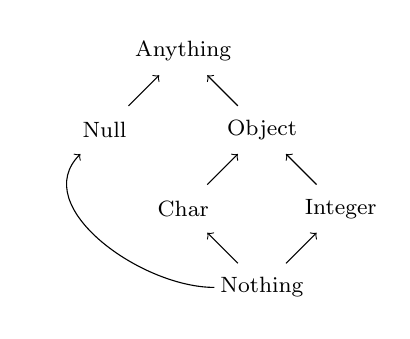
\begin{tikzpicture}[<-]
  \footnotesize
  \node[state, anchor=center] (a) at (0, 0) {Null};
  \node[state, anchor=center] (b) at (2, 0) {Object};
  \node[state, anchor=center] (c) at (1, 1) {Anything};
  \node[state, anchor=center] (d) at (1, -1) {Char};
  \node[state, anchor=center] (e) at (3, -1) {Integer};
  \node[state, anchor=center] (f) at (2, -2) {Nothing};
  \draw (c) -- (a);
  \draw (c) -- (b);
  \draw (b) -- (d);
  \draw (b) -- (e);
  \draw (e) -- (f);
  \draw (d) -- (f);
  \draw (a) to[out=225,in=180] (f);
\end{tikzpicture}
\end{center}
\caption{Ceylon's subtyping hierarchy. Note that \lstinline{Null} only has \lstinline{Nothing} as its subtype.}
\label{fig:null}
\end{figure}

In Ceylon the following code:

\begin{lstlisting}[language=Scala]
  String str = null;
\end{lstlisting}

\noindent is rejected with a type error, since \lstinline{null} cannot have type \lstinline{String}.
Instead, a type that can have the null value must be defined explicitly
in Ceylon using union types:

\begin{lstlisting}[language=Scala]
  String | Null str = null;
\end{lstlisting}

\noindent Now we cannot call \lstinline{str.size},
as \lstinline{str} may be \lstinline{null}, and \lstinline{size} is not defined
on \lstinline{null}.
To get the \lstinline{size} of \lstinline{str}, we must first check whether \lstinline{str} is \lstinline{null}
or not using disjoint switches:
% \bruno{Please show valid Ceylon code using switches here! We do not need to adapt anything from Scala:
%   Ceylon has this feature, just show valid Ceylon code that illustrates this feature! Make sure
% that all the code in Section 2.3 and 2.4 is valid Ceylon code.}

\begin{lstlisting}[language=Scala]
  String | Null str = null;
  switch (str)
    case (is String) { print(str.size); }
    case (is Null)   { print(); }
\end{lstlisting}

%\baber{Scala does not support Null type in switch construct.}
\paragraph*{Other uses of Union Types.}
Union types are also useful in many other situations.
In Section~\ref{subsec:elimination} we illustrated a \lstinline{safediv} operation, which
can be easily encoded in Ceylon as:
%
\begin{lstlisting}[language=Scala]
  String | Integer safediv3 (Integer x, Integer y){
    if (y==0) { return "Divided by zero"; }
    else      { return (x/y); }
  }
\end{lstlisting}
%
The return value can be a string or an integer,
with no explicit tag needed,
as union types are implicitly introduced.
As long as the declared return type of the function
is a supertype of all possible return values, it is valid
in Ceylon.





%Similarly, one can use enumerated types to denote various special cases, or easily
%add another type to the argument type of an existing function when considering
%more possible inputs, to improve the program's robustness.
%Next, we will see how Ceylon's static type checking helps programmers.

\begin{comment}
\paragraph*{Exhaustiveness}

Ceylon checks the exhaustiveness of a switch by comparing the union of all
cases and the switched term's type.
For the switch to be accepted, the former must be a supertype of the later.
%Recall that adding more components to a union type make it a supertype of the
%initial type, like \lstinline{Integer|Float} to \lstinline{Integer}.
That is to say a switch construct must have enough cases to handle all
possible runtime types of the term.
%
For example, here we define \lstinline{Node} by enumerating its subtypes.
It can be viewed as the union of \lstinline{Leaf} and \lstinline{Branch}.
Then in the function \lstinline{printTree} that takes a \lstinline{Node},
both cases are taken into consideration.
%
\begin{comment}
------------- THE OTHER EXAMPLE -----------------
Adding more subtype in it causes error in exhaustiveness checking in switch.
\begin{lstlisting}
interface Resource of File | Directory | Link { }
interface File satisfies Resource {}
interface Directory satisfies Resource {}
interface Link satisfies Resource {}

void printType(Resource resource){
	switch (resource)
	case (is File) { print("File"); }
	case (is Directory) { print("Directory"); }
	case (is Link) { print("Link"); }
}
\end{lstlisting}

%
\begin{lstlisting}
abstract class Node() of Leaf | Branch {}

class Leaf(shared Object element)
extends Node() {}

class Branch(shared Node left, shared Node right)
extends Node() {}

void printTree(Node node) {
	switch (node)
	case (is Leaf) {
		print("Found a leaf: ``node.element``!");
	}
	case (is Branch) {
		printTree(node.left);
		printTree(node.right);
	}
}

printTree(Branch(Branch(Leaf("aap"), Leaf("noot")), Leaf("mies")));
\end{lstlisting}
% https://ceylon-lang.org/documentation/1.3/tour/types/
%
We can allow the input to be \lstinline{null} by replacing the argument type \lstinline{Node} by \lstinline{Node?}.
Ceylon uses union types to encode nullable types (or the optional types) in a
type-safe way.
The null value is inhabited in \lstinline{Null}, and \lstinline{A?} stands for \lstinline{A|Null}.
If the switched term has a nullable type, the exhaustive checking makes sure there
is a branch to handle it.
%
Similarly, one can use enumerated types to denote various special cases, or easily
add another type to the argument type of an existing function when considering
more possible inputs, to improve the program's robustness.
%
If we can add more subtype in the declaration of \lstinline{Node} without
adapting the function definition, an compiling error will be raised:
case types must cover all cases of the switch type.
Such checking reminds programmers to keep consistent when changing the
related code and avoid potential runtime errors.

\bruno{The following example is better, and I guess useful to illustrate exhaustiveness.}
\begin{lstlisting}
	void printAfterPlusOne(Integer|String x) {
		switch (x)
		case (is Integer|Float) { print(x+1); }
		case (is String) { print("String:"+x); }
	}
\end{lstlisting}
%
Exhaustiveness checking does not prevent the cases in a switch to
accept more than necessary.
For example, in the above function, even though \lstinline{x} cannot be
a \lstinline{Float}, it is not harmful for the first branch to expect
a term of \lstinline{Integer|Float}, since \lstinline{Integer|Float|String}
still covers \lstinline{Integer|String}.


\paragraph*{Disjointness}
Ceylon prevents any pair of cases in a switch from overlapping.
And disjointness is introduced to describe such relation between two types.
Being disjoint means the non-existence of a value which can be assigned to
both types.
With the existence of subtyping, a branch in switch/case expression
can take a term of a subtype of its expected type.
Therefore disjointness roughly equals to no common subtype.
However, this does not directly lead to an algorithm. So Ceylon
provides a set of rules: 1) distinct cases in an enumerated type is thought to
be disjoint, and their subtypes are disjoint too; 2) two classes, if they are
not subclass of each other, are disjoint; and etc.
Especially, for a union type $[[A1\/A2]]$, being disjoint with another
type $B$ requires both $[[A1]]$ and $[[A2]]$ to be disjoint with $B$.
Eventually, after decomposing and examining subtyping relation, it is decidable
that two types are disjoint or not.

% https://github.com/ceylon/ceylon-spec/issues/50
% https://github.com/ceylon/ceylon-spec/issues/65

Disjointness is the foundation of
Ceylon's deterministic and order-irrelevant semantics of the switch construct.
Forcing all cases to be disjoint eliminates ambiguity, and avoid subtle bugs that may arise from overlapping cases.
%
People may argue that the programmer should be free to use overlapping cases
and arrange their order intentionally. The following example provides a scenario
where the programmer may not notice the dangerous overlapping.
%
\begin{lstlisting}
	alias Number => Integer | Null;
	String getNumber(Number n) {
		switch (n)
		case (is Integer) { return "``n``"; }
		case (is Null) { return "infinity"; }

	}
	void  printAge(Number|Null x) {
		switch (x)
		case (is Number) { print("Age is ``getNumber(x)``".); }
		case (is Null) { print("Age is not provided."); }
	}
\end{lstlisting}
%
Assume \lstinline{Number} is already defined where \lstinline{null} stands for
infinity. A client uses it to store age information.
Meanwhile, the client use \lstinline{null} to denote missing data.
Without disjointness checking, the above code will be accepted.
But in \lstinline{printAge}, the second branch is always shadowed by the first one.
Any missing data will be interpreted as infinity.
%
Note that swapping the two cases cannot prevent all unexpected behaviors.
In that case the meaning of infinity is hidden.
On contrary, disjoint cases are always distinguishable, and the user, when
using an existing definition, is guaranteed that there is no hidden conflicts.

\paragraph*{the bottom type}
To dig deeper for disjointness, it often comes to the the concept
of \emph{bottom type}.
Bottom type is a subtype of all types, in contrast to the top type.
Certainly the bottom type has no value.
In Ceylon, it is called \lstinline{Nothing}, representing the empty set.
%
For two disjoint types $[[A]]$ and $[[B]]$, their intersection $[[A/\B]]$
is naturally a common subtype, and therefore must be equivalent to
the bottom type \lstinline{Nothing}.
\end{comment}

\begin{comment}
\paragraph*{Existing problems in Ceylon}
In general, a term of type $A$ is always assignable to any supertype of $A$.
But in Ceylon, the checking of assignability is not complete to
subtyping.
Although the subtyping relation holds between \lstinline{v}'s
(declarative) type and \lstinline{Integer}, \lstinline{v}
is not assignable to \lstinline{Integer}, and the following program
cannot be accepted by Ceylon's compiler.
% https://try.ceylon-lang.org/#

\begin{lstlisting}
	< Character | Integer > & < String | Integer > v = 100;
	switch (v)
	case (is Integer) { print("Integer: ``v``"); }
\end{lstlisting}
\end{comment}


%---------------------------------------------------%%

%%%%%%%%%%%%%%%%%%%% Polymorphism %%%%%%%%%%%%%%%%%%%%

%---------------------------------------------------%%


\section{Polymorphism}

Polymorphism is an essential feature supported in almost all the modern
programming languages. The word polymorphism can map to three
important concepts in programming languages. This includes
subtype polymorphism, ad-hoc polymorphism 
\citep{castagna1995calculus, cardelli1985understanding, wadler1989make} and 
parametric polymorphism \citep{cardelli1985understanding, canning1989f}. 
In our current setting polymorphism refers to
parametric polymorphism.
It enables generic programming by abstracting over types not just terms.
Parametric polymorphism lies at the core of most functional programming languages
including Haskell and Ocaml among others. The following programming example
illustrates parametric polymorphism:

\begin{lstlisting}[language=Scala]
  Int length [T] (l Array[T]) {}
\end{lstlisting}

\noindent Length is a generic function which calculates the size
of array of any type. It does not depend on the type of the
elements in an array, it only cares about the number of elements.
In a programming language where parametric polymorphism is not
supported one may have to write multiple length functions dealing
with one type each. Parametric polymorphism can further be 
refined using bounded quantification
to restrict the instantiation of type variables to be subtype of
certain types. For example:

\begin{lstlisting}[language=Scala,mathescape]
  Int length$'$ [T <: Number] (l Array[T]) {}
\end{lstlisting}

\noindent The function \emph{length$'$} type-checks as long as the type
variable T is a subtype of Number.
We discuss a variant of parametric polymorphism called
the disjoint polymorphism in \Cref{sec:poly} and
\Cref{chap:disjointness}. Disjoint polymorphism
poses a disjointness restriction on type variables
instead of subtyping restriction. This is illustrated by
the following example:

\begin{lstlisting}[language=Scala]
  Bool isstudent [T * Student] (x: T | Student) = switch (x)
                                           (y : T)       -> false
                                           (y : Student) -> true
\end{lstlisting}

\noindent The function \lstinline{isstudent} is abstracted over types.
Type variable \lstinline{T} has a disjointness constraint.
It can be instantiated by any type
given that the type is disjoint to \lstinline{Student}.
Disjoint polymorphism is essential for polymorphic disjoint
switches. This will further be discussed in \Cref{sec:poly} and
\Cref{chap:disjointness}.


%---------------------------------------------------%%

%%%%%%%%%%%%%%%%%%%%%% Duality %%%%%%%%%%%%%%%%%%%%%%%

%---------------------------------------------------%%


\section{Duality}
%\baber{Need to revise this section.}
Duality is a common concept in logic. Many features and 
their duals have been studied.
Modal logic \citep{simpson1994proof,nanevski2008contextual} studies 
duality between necessity and possibility.
Necessity is dual to possibility in a sense 
that necessity must always
hold, whereas the possibility may not always hold.
Similarly, conjunctions and disjunctions are 
known to be dual features in logic.
Duality of conjunction and disjunction is 
shown by De Morgan's laws \citep{copi2018introduction} as:
(where A and B are propositions)
%\baber{add citation for De Morgan's law.}

\begin{center}
  $[[A /\ B]]$ $\equiv$ $\neg$ ($\neg$ $[[A]]$ $[[\/]]$ $\neg$ $[[B]]$)
\end{center}

\noindent and

\begin{center}
  $[[A \/ B]]$ $\equiv$ $\neg$ ($\neg$ $[[A]]$ $[[/\]]$ $\neg$ $[[B]]$)
\end{center}

\noindent Similarly, universal and existential quantifiers are known to be
dual in logic.

\begin{center}
  $\forall$ x . $[[A]]$ $\equiv$ $\neg$ $\exists$ x . $\neg$ $[[A]]$
\end{center}

\noindent Conversely, the other dual equality is written as:

\begin{center}
  $\exists$ x . $[[A]]$ $\equiv$ $\neg$ $\forall$ x . $\neg$ $[[A]]$
\end{center}

There is also a strong connection between conjunction and universal quantifier
and disjunction and the existential quantifier. Universal quantifier can be
thought as conjunction of infinite propositions. Whereas, existential quantifier
can be though as disjunction of infinite propositions. Since propositions are types
as per the Curry–Howard correspondence \citep{curry1958combinatory, howard1980formulae}.
This points to a study of the duality
among types. Intersection types and union types are the dual features
in the theory of programming languages. In particular, we study the
duality in the subtyping of intersection types and union types in this thesis.


% \paragraph*{Duality in subtyping.}
% In a system with both supertyping and subtyping,
% the top and bottom subtyping rules can be presented as follows:

% \begin{center}
%   \begin{tabular}{lll}
%     \drule{s-top} & & \drule{sup-bot}
%   \end{tabular}
% \end{center}

% \noindent Close analysis of \rref{s-top,sup-bot} reveals that only difference
% in these two rules is the relation. Depending upon the relation upper and lower
% can be selected. If the relation is subtyping ($[[<:]]$) upper bound is top,
% if the relation is supertyping ($[[:>]]$) lower bound is bottom.
% It turns out that these two rules can be composed in one unified rule as:

% \begin{center}
%        \drule[]{gds-topbot}
% \end{center}

% where $[[duo]]$ is the mode and is defined as:

% \begin{center}
% \begin{tabular}{lrcl}
%   Mode & $[[duo]]$  & $\Coloneqq$ & $[[msub]] \ \mid \ [[msup]]$
% \end{tabular}
% \end{center}

% \noindent which can be subtyping ($[[msub]]$) or supertyping ($[[msup]]$).
% If the mode is subtyping the upper bound of the relation is 
% the top type, otherwise it is
% the bottom type. With $\rceil [[duo]] \lceil$ we can then write a single unified
% \rref{gds-topbot} that captures the upper bounds of subtyping and supertyping, 
% and which generalizes both \rref{s-top} and \rref{sup-bot}.
% $\rceil [[duo]] \lceil$ is a function which returns either top as upper bound
% or bottom as lower bound depending the specific mode value.


% While such dual features have been studied in logic and linguistic.
% To our best knowledge, there has not been any formalization to exploit
% the duality among certain features in the context of subtyping in
% programming languages.
% We formally study the duality of subtyping in this
% thesis in \cref{chap:duo}.

%\baber{Research idea: Come with a dual subtyping rule for existential
%and universal quantifier.}


%%% Local Variables:
%%% mode: latex
%%% TeX-master: "../Thesis"
%%% org-ref-default-bibliography: "../Thesis.bib"
%%% End:
